\section{Introduction}
\label{sec:introduction}

% state the learning objective 

\hspace{0,5cm} This report is being made for the subject of Circuit Theory and Electronics Fundamentals and is related to the fifth laboratory being its objective to develop a Bandpass Filter using OP-AMP. In this laboratory there are some specifications that are followed such as a central frequency of 1kHz and a gain at central frequency of 40dB. There are also limited numeber of the different components. Ass in all, the circuit that was implemented is shown in figure \ref{fig:circuito}.
\par In Section~\ref{sec:analysis} a theoretical analysis will be made . Secondly, in Section~\ref{sec:simulation} it will be simulated the circuit using ngspice tools. Following with both results from Section~\ref{sec:analysis} and Section~\ref{sec:simulation} being compared and commented in Section ~\ref{sec:comparison}. 
\par Also, it is important to notice that the NGSpice simulation was made using the provided OPAMP model
\par Finally, the conclusions of this study are outlined in Section~\ref{sec:conclusion}.

\begin{figure}[H] \centering
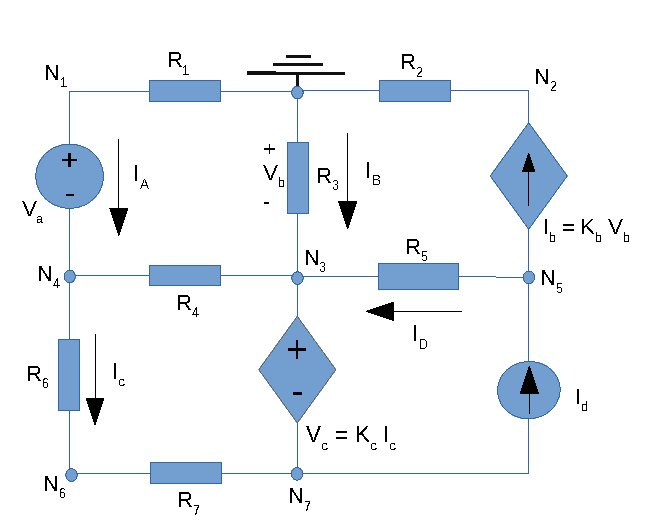
\includegraphics[width=1\linewidth]{circuito.pdf}
\caption{Audio Amplifier Circuit}
\label{fig:circuito}
\end{figure}


